\documentclass[10pt,twocolumn]{witseiepaper}

%
% All KJN's macros and goodies (some shameless borrowing from SPL)
\usepackage{KJN}
\usepackage{subcaption}
\usepackage{listings}
\usepackage{amsmath}
\usepackage{epstopdf}
\usepackage{xcolor}
\usepackage{textcomp}
\usepackage{listings}
\usepackage{alltt}
\usepackage{matlab-prettifier}
\usepackage{graphicx}
\usepackage{changes}
\usepackage{makecell}
\usepackage{verbatim}
\usepackage[super]{nth}
\usepackage{algorithm,algpseudocode}
\usepackage{mathtools, cuted}
\usepackage{stfloats}% <-- added
\usepackage{balance}
\usepackage[font=small]{caption}
\usepackage{color} %red, green, blue, yellow, cyan, magenta, black, white
\definecolor{mygreen}{RGB}{28,172,0} % color values Red, Green, Blue
\definecolor{mylilas}{RGB}{170,55,241}
%\usepackage{flafter}

\lstset{language=Matlab, % Set colour for matlab code
	breaklines=true,%
	morekeywords={matlab2tikz},
	keywordstyle=\color{blue},%
	morekeywords=[2]{1}, keywordstyle=[2]{\color{black}},
	identifierstyle=\color{black},%
	stringstyle=\color{mylilas},
	commentstyle=\color{mygreen},%
	showstringspaces=false,%without this there will be a symbol in the places where there is a space
	numbers=left,%
	numberstyle={\tiny \color{black}},% size of the numbers
	numbersep=9pt, % this defines how far the numbers are from the text
	emph=[1]{for,end,break},emphstyle=[1]\color{red}, %some words to emphasise
	%emph=[2]{word1,word2}, emphstyle=[2]{style},    
}


%
% PDF Info
%
%%%%%%%%%%%%%%%%%%%%%%%%%%%%%%%%%%%%%%%%%%%%%%%%%%%%%%%%%%%%%%%%%%%%%%%%%%%%%%%
\begin{document}


\title{PROJECT PLAN FOR THE DESIGN AND IMPLEMENTATION OF AN ADAPTIVE HEARING AID}

\author{Kayla-Jade Butkow (714227) \& Kelvin da Silva (835842) 
\thanks{School of Electrical \& Information Engineering, University of the
Witwatersrand, Private Bag 3, 2050, Johannesburg, South Africa}
}


%%%%%%%%%%%%%%%%%%%%%%%%%%%%%%%%%%%%%%%%%%%%%%%%%%%%%%%%%%%%%%%%%%%%%%%%%%%%%%%
%
\abstract{ }

\keywords{}

\maketitle
\thispagestyle{empty}
\pagestyle{plain}
\setcounter{page}{1}

%%%%%%%%%%%%%%%%%%%%%%%%%%%%%%%%%%%%%%%%%%%%%%%%%%%%%%%%%%%%%%%%%%%%%%%%%%%%%%%
%
\section{INTRODUCTION}
clarify what the hearing aid is
\section{PROJECT SPECIFICATIONS}
\subsection{Problem Analysis}
\subsection{Requirements and Specifications}
\subsection{Assumptions}
assuming we can use the kudu wave
\subsection{Success Criteria}
\subsection{Constraints}

\section{PROJECT BACKGROUND}
\subsection{Literature Review}
The aim of the filter bank is to divide the audible frequency range into a number of bands, so that different amplifications can be applied to different ranges.

\section{SYSTEM DESIGN}

A block diagram of the full system is given in \figref{fig:block}.

\begin{figure*}[t]
	\centering
	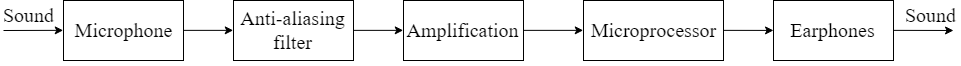
\includegraphics[width=1\textwidth]{highLeveLSystemDiagram.png}
	\caption{Full system block diagram}
	\raggedright
	\label{fig:block}	
\end{figure*}

The microprocessor block consists of all of the signal processing required for the functioning of the hearing aid. The required signal processing is expanded upon in \figref{fig:microBlock}.


\begin{figure*}[t]
	\centering
	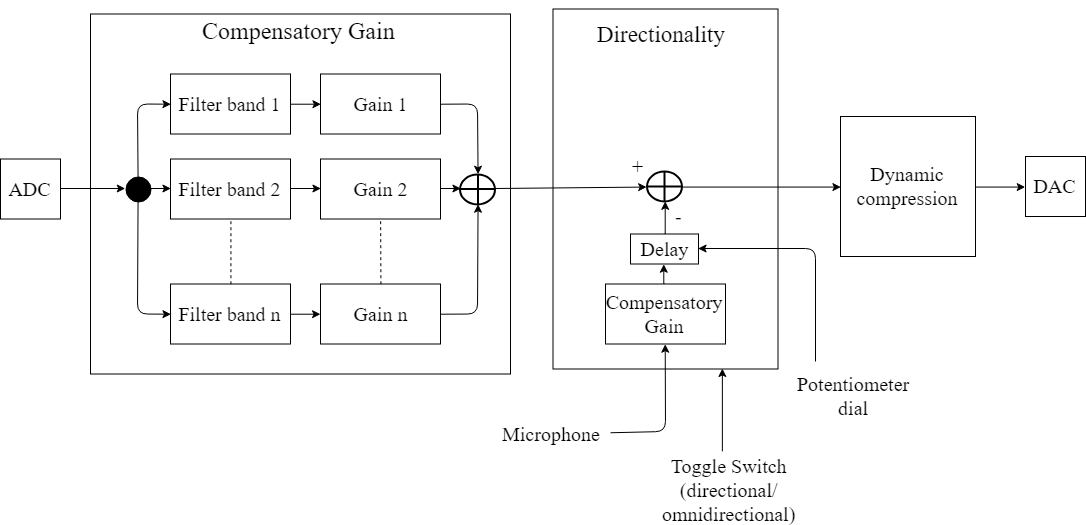
\includegraphics[width=0.8\textwidth]{microBlockDiagrm.png}
	\caption{Block diagram of the }
	\raggedright
	\label{fig:microBlock}	
\end{figure*}

\subsection{Compensatory Amplification}

\subsection{Directionality}

\subsection{Hardware} \label{sec:hardware}
Analog circuitry is required to acquire the sound signal, condition it and convert it to digital. To acquire the signal, two omni-directional microphones are used. The front microphone is the primary microphone and is used alone when the omni-directional mode is selected. The rear microphone is used when directional mode is selected. The signals from the microphones are amplified and then passed through an anti-aliasing filter. The filter has a cutoff frequency of 25~kHz

The circuit includes the microphone, audio amplifier, anti-aliasing filter, microprocessor (for analog to digital conversion and digital to analog conversion). The circuit also includes a potentiometer, which acts as a dial to tune the directionality of the hearing aid. Furthermore, the hearing aid will include a power button to turn the device on or off, and a toggle switch to switch between directional and omni-directional amplification modes. The resultant sound will be relayed to the user using headphones which interact with a headphone jack. The entire system will be powered using rechargeable batteries. A preliminary circuit diagram of the hardware component of the system is given in \figref{fig:circuit}.

\begin{figure}[h]
	\centering
	%	\includegraphics[width=1\columnwidth]{}
	\caption{Circuit diagram for the system}
	\raggedright
	\label{fig:circuit}	
\end{figure}

\subsection{Laboratory Full System Testing} \label{sec:laboratory}
In order to obtain objective results that are free from human bias, the system will be tested in a laboratory using a signal generator to generate pure tones. By generating pure tones of specific frequencies and feeding these tones to the hearing aid, the ability of the device to apply compensatory amplification, and to apply amplification to the correct frequencies, can be quantified. The frequency of the sinusoidal pure tone signals will be set to range from the lower to the upper bounds of the frequency range of human hearing. Additionally, high frequency noise will be added to the signals such that the performance of the device can be evaluated in the presence of noise.

In order to test the directionality of the device, one speaker will be placed in a fixed position. The hearing aid will be placed in the centre of a rotating platform with the dial facing towards the speaker. A pure tone signal is played from the speaker and the resulting output signal from the hearing aid is saved. The platform is then rotated by 5\textdegree and the procedure is repeated. This is done for 360\textdegree. Once signals have been acquired corresponding to each 5\textdegree increment, a polar plot of the signals will be created. In the polar plot, the angle of the signals is taken as the angle of the hearing aid relative the dial (the 0\textdegree reference point). This will allow for an analysis of the degree of amplification and attenuation of signals in all directions with the directionality being fixed in one direction.

\subsection{Clinical Full System Testing} \label{sec:clinical}
In order to verify the performance of the hearing aid, clinical tests are required. This will allow for a quantification of the value that the hearing aid provides to the participant.

The method of the clinical testing will now be detailed. First, staff from the school of Electrical and Information Engineering will be asked to participate in the clinical testing. Prior to performing the tests, an audiogram will be collected from each participant using the KUDUwave headset. A hearing aid will then be customised for each participant. Thereafter, a second audiogram will be obtained with the participant wearing the hearing aid. Since the KUDUwave cannot be used on top of earphones, the microphone will be mounted on a model head (made out of polystyrene) and the KUDUwave headset will be placed on top of the fake head. The participant will then wear the earphones which receive the processed signals and a second audiogram will be obtained. The two audiograms will then be compared in order to assess the effectiveness of the compensatory amplification in the device.

\begin{figure}[h]
	\centering
	\begin{subfigure}[t]{0.5\textwidth}
		\centering
		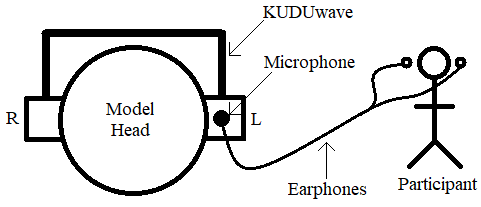
\includegraphics[width=0.8\columnwidth]{gainTestingLeft.png}
		\caption{Testing the left ear}
	\end{subfigure}%
	\\
	\begin{subfigure}[t]{0.5\textwidth}
		\centering
		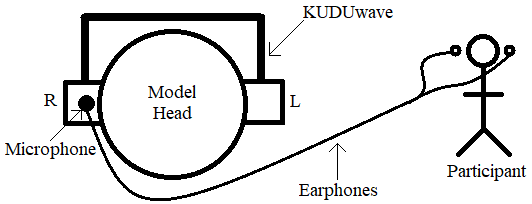
\includegraphics[width=0.8\columnwidth]{gainTestingRight.png}
		\caption{Testing the right ear}
	\end{subfigure}
	\caption{Schematic of the procedure for testing compensatory amplification}
	\label{fig:testing}	
\end{figure}

In order to test the directionality of the device, eight speakers will be set up in a circle, separated by 45$\textdegree$ angles. The participant will be asked to sit in a chair which faces 0$\textdegree$ while wearing the hearing aid. Pure tone sounds will be played from a single speaker at a time and the participant will be asked to tune the dial controlling the directionality until the sound is at its loudest. The angle of the dial will then be recorded and compared to the angle of the speaker, thus allowing for a quantification of the error present in the directionality. 

\section{PROJECT METHODOLOGIES AND MANAGEMENT}
\subsection{Project Phases}
The project has been divided into 11 development phases, which encapsulate the entire project, from ethics clearance to the presentation. Three of these phases occurred prior to the submission of this document. The phases are detailed in the following sections.

\subsubsection*{Phase 1: Obtain Ethics Clearance} $    $

This phase involved obtaining ethics clearance for the project. This clearance is necessary for clinical testing of the hearing aid, using human input. The procedure for obtaining clearance involves setting out the testing procedure, creating consent forms and creating the questionnaire's for the participants to complete. This phase was completed between the \nth{29} March and the \nth{6} April. Ethics clearance was granted on the \nth{11} May. Both partners were involved in the completion of this phase.

\subsubsection*{Phase 2: Research} $    $

This phase involved performing the research for the project. This included research into compensatory gain, directionality, filtering and the conversion of digital signals to sound signals. This phase occurred from the \nth{25} June to the \nth{1} July. However, it must be noted that research will be an ongoing process throughout the entire duration of the project. Kayla-Jade performed research into gain and filtering and Kelvin investigated directionality and conversions. Thereafter, the research was shared and both partners familiarised themselves with both sets of research.

\subsubsection*{Phase 3: Hardware Design } $    $

In this phase, the circuit diagrams required in the project were designed. The overall system circuit diagram is given in \figref{fig:circuit}. This phase was completed between the \nth{2} July and the \nth{6} July. The two partners performed this phase together.

\subsubsection*{Phase 4: Construction of Hardware } $    $

This phase involves the construction of the circuit that was designed in Phase 3. The circuit will be prototyped on a breadboard before being finalised on a PCB board. The phase will begin on the \nth{9} of July and will end on the \nth{16}. Kelvin will perform the construction of the hardware.

\subsubsection*{Phase 5: Implementation of Compensatory Amplification} $    $

In this phase, the compensatory amplification aspect of the hearing aid will be implemented. This phase has numerous sub-phases:
\begin{itemize}
	\item Sub-phase 1: Interpolation of audiograms 
	\item Sub-phase 2: Development of the filter bank
	\item Sub-phase 3: Designing the gains for each filter based on the audiogram
	\item Sub-phase 4: Attack and release times for changing the gain per frequency range 
	\item Sub-phase 5: Dynamic compression of signals
	\item Sub-phase 6: Optimisation of code from the previous stages to allow for real-time signal processing
\end{itemize}

In sub-phase 1, the data from the audiogram will be hard-coded onto MATLAB, and will be linearly interpolated to increase resolution. In sub-phase 2, the filter bank for the auditory compensation will be designed and implemented. 
**** Come back here!!! ****

The first two sub-phases will be implemented concurrently with phase 4 by Kayla-Jade. Thereafter, sub-phases 3 and 4 will be implemented by Kayla-Jade, while Kelvin concurrently implements sub-phases 5 and 6.


\subsubsection*{Phase 6: Implementation of the Software Required for Directionality} $    $

In this phase, the software required to implement directionality will be implemented. This software will interface with the dial built into the hardware to tune the direction in which the sound must be amplified. The two partners will implement this phase together. 
*** Date ***

\subsubsection*{Phase 7: Laboratory testing of the full system} $    $

Following the implementation of the entire system, full system testing is required. 

Both partners will perform the laboratory testing.

\subsubsection*{Phase 8: Clinical testing of the full system} $    $

Phase 7 involves the testing of the audiogram in a clinical setting, using human participants. The procedure to be implemented in this phase is that described in \secref{sec:clinical}

Both partners will perform the clinical testing.

\subsubsection*{Phase 9: Demonstration} $    $

This phase involves the preparation for open day. This includes creating a poster and a video explaining the project. It also includes preparing the demonstration for open day. Both partners will be involved in all aspects of the phase.

\subsubsection*{Phase 10: Documentation} $    $

This phase involves the writing of the final project report. The report will be worked on throughout the entire project, but in this phase, it will be the sole focus. The partners will each work on their reports individually.

\subsubsection*{Phase 11: Presentation} $    $
Phase 11 is the final phase of the project which involves the preparation of the presentation. This will be done by the partners together.

\section{CONCLUSION}


\bibliographystyle{witseie}
\bibliography{labproject}

\end{document}